\documentclass[conference,a4paper]{IEEEtran}
\pdfminorversion=6
\IEEEoverridecommandlockouts

\usepackage{cite}
\usepackage{amsmath,amssymb,amsfonts}
\usepackage{graphicx}
\usepackage{textcomp}
\usepackage{booktabs}
\usepackage{multirow}
\usepackage{array}
\usepackage[table]{xcolor}
\usepackage{pifont}
\usepackage{hyperref}
\usepackage{listings}
\usepackage{balance}
\usepackage{placeins}
\usepackage{tikz}
\usepackage{pgfplots}
\pgfplotsset{compat=1.18}
\usetikzlibrary{shapes.geometric, arrows.meta, positioning, calc, fit, backgrounds}

\definecolor{checkgreen}{HTML}{2E7D32}
\definecolor{crossred}{HTML}{C62828}
\definecolor{ourgreen}{HTML}{E8F5E9}
\definecolor{headergray}{HTML}{ECEFF1}
\definecolor{accentblue}{HTML}{1565C0}
\definecolor{boxgray}{HTML}{F8F9FA}

\newcommand{\cmark}{\textcolor{checkgreen}{\ding{51}}}
\newcommand{\xmark}{\textcolor{crossred}{\ding{55}}}

\lstdefinestyle{promptstyle}{
  basicstyle=\ttfamily\scriptsize,
  backgroundcolor=\color{boxgray},
  frame=single,
  rulecolor=\color{black!30},
  breaklines=true,
  columns=fullflexible,
  keepspaces=true,
  xleftmargin=1.5mm,
  xrightmargin=1.5mm
}

\def\BibTeX{{\rm B\kern-.05em{\sc i\kern-.025em b}\kern-.08em
    T\kern-.1667em\lower.7ex\hbox{E}\kern-.125emX}}

\begin{document}

\title{SymPlan: Enhancing Neurosymbolic Mathematical Reasoning in SLMs via Representation and Planning}

\author{
Tay Bui\textsuperscript{1,2},
Huy N. G. Pham\textsuperscript{1,2},
Nhan Ha Le Thanh\textsuperscript{3}\\
\textsuperscript{1} University of Information Technology, Ho Chi Minh City, Vietnam\\
\textsuperscript{2} Vietnam National University, Ho Chi Minh City, Vietnam\\
\textsuperscript{3} FPT University, Ho Chi Minh City, Vietnam\\
\texttt{\small \{24521589, 24520690\}@gm.uit.edu.vn},
\texttt{\small hnhan5355@gmail.com}
}

\maketitle

\nocite{wei2022cot}
\nocite{gao2023pal}
\nocite{chen2022pot}
\nocite{nezhad2025symcode}
\nocite{meurer2017sympy}
\nocite{yang2024qwenmath}
\nocite{he2024olympiadbench}
\nocite{cobbe2021gsm8k}
\nocite{wang2023plan}

\begin{abstract}
Mathematical reasoning with language models increasingly relies on executable symbolic programs, yet reliability remains elusive when compact models must translate a natural-language problem directly into code. The core difficulty is not only computation, but formulation: a syntactically valid program may still miss hidden constraints, choose an invalid branch, or collapse under the mixed grammar of prose, mathematics, and code. This limitation is particularly severe for small language models, causing monolithic approaches such as SymCode to exhibit frequent formulation, constraint-omission, and code-generation errors. We introduce SymPlan, a structured neurosymbolic framework that separates symbolic problem solving into structured problem representation, algorithmic planning, and plan-guided SymPy generation. By making variables, targets, and domain constraints explicit before code synthesis and carrying them into the generated program, SymPlan turns fragile one-shot generation into a more inspectable reasoning pipeline. Across MATH-500 and GSM8K, SymPlan consistently improves answer accuracy while maintaining high execution reliability, with particularly clear gains against monolithic SymPy generation. These results suggest that the next step for small language models is not merely larger computation, but more disciplined interfaces between informal mathematical intent and formal symbolic execution.
\end{abstract}

\begin{IEEEkeywords}
Neurosymbolic Reasoning, Mathematical Problem Solving, Small Language Models, SymPy Code Generation, Structured Problem Representation, Algorithmic Planning.
\end{IEEEkeywords}

\section{Introduction}

Large Language Models (LLMs) have demonstrated strong capabilities in complex reasoning tasks, with Chain-of-Thought (CoT) prompting improving their ability to perform multi-step reasoning~\cite{wei2022cot}. Subsequent methods improve robustness by sampling multiple reasoning paths, decomposing difficult questions into simpler subproblems, or constructing an explicit plan before solving~\cite{wang2023selfconsistency,zhou2023leasttomost,wang2023plan}. However, autoregressive mathematical reasoning remains susceptible to calculation errors, missing reasoning steps, and semantic misunderstandings, making intermediate solutions difficult to reliably inspect or verify~\cite{lyu2023faithful,he2024olympiadbench}.

Program-aided approaches address these limitations by delegating computation to executable programs. Program-Aided Language Models (PAL)~\cite{gao2023pal} and Program-of-Thought (PoT)~\cite{chen2022pot} separate reasoning from computation by using external interpreters for numerical operations. MathCoder and ToRA further integrate natural-language reasoning with code execution and mathematical tools~\cite{wang2024mathcoder,gou2024tora}. More recently, SymCode~\cite{nezhad2025symcode} extends this paradigm to symbolic mathematics by generating executable programs with the SymPy symbolic computation library~\cite{meurer2017sympy}, enabling mathematical solutions to be checked through program execution.

\begin{figure*}[t]
\centering
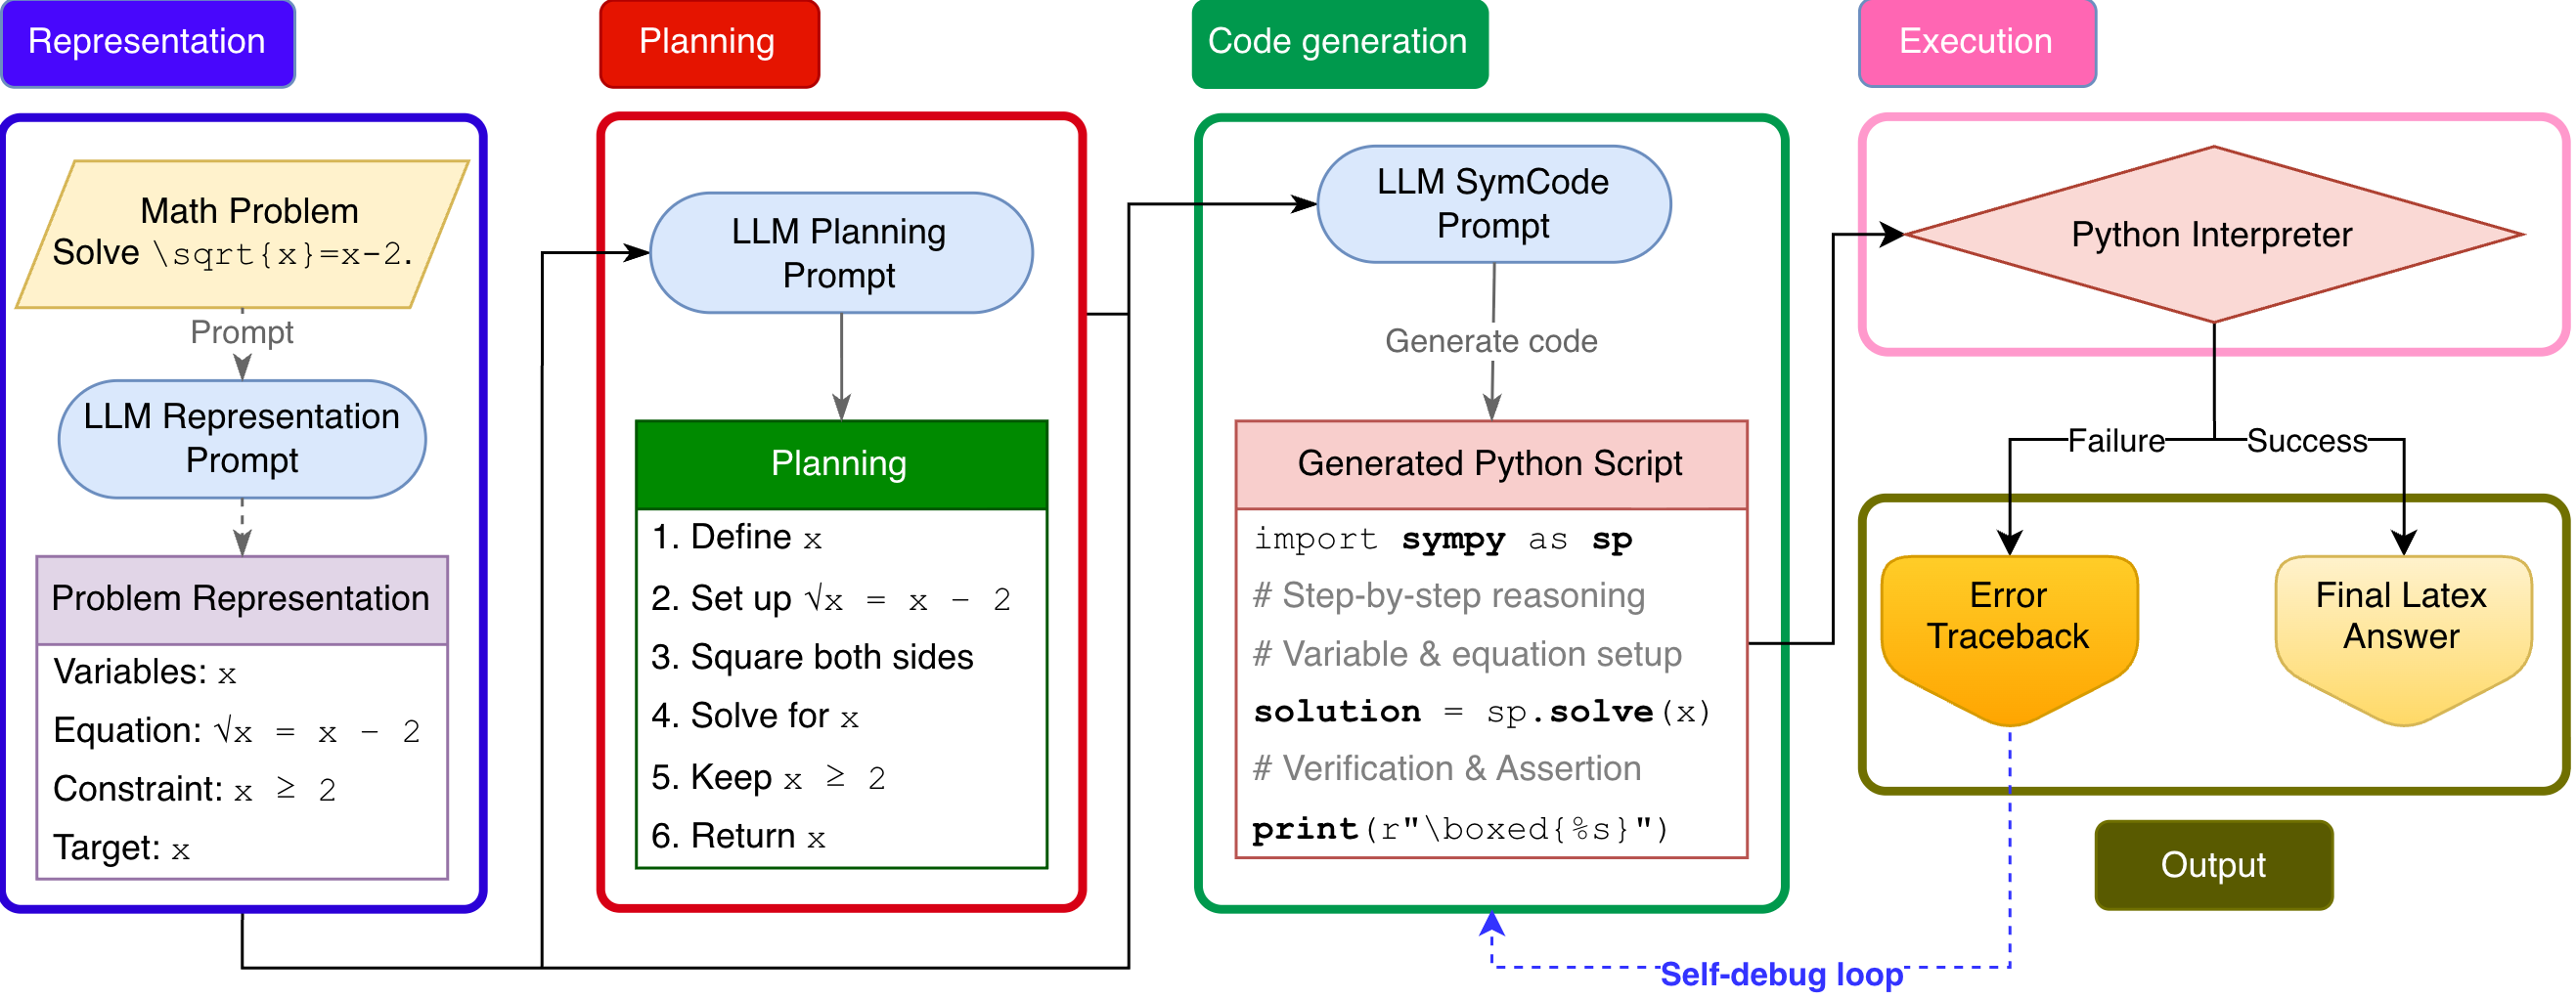
\includegraphics[width=\textwidth]{pipeline-symplan.png}
\caption{Overview of SymPlan. A problem is transformed into a structured representation and an explicit plan before SymPy code generation. The script is executed by a Python interpreter; failures return a traceback to code generation, while successful runs produce a final \LaTeX{} answer.}
\label{fig:overview}
\end{figure*}

Despite these advances, program execution alone does not guarantee correct problem interpretation. Translation-based neurosymbolic systems likewise depend on the correctness of the generated formalization before a deterministic solver is invoked~\cite{lyu2023faithful,pan2023logiclm}. Existing program-aided approaches often couple problem understanding, solution reasoning, and program synthesis within a single generation process. Consequently, a program may be syntactically valid and execute successfully while encoding an incorrect mathematical formulation. This issue is particularly challenging for compact language models, which must simultaneously interpret the problem, construct a solution strategy, and synthesize formal symbolic code. Although decomposition and planning can reduce missing-step errors~\cite{khot2023decomposed,zhou2023leasttomost,wang2023plan}, they have not been systematically connected to structured mathematical representation and SymPy generation for compact models.

To investigate these limitations, we conduct a systematic failure analysis across three compact language models---Qwen2.5-Coder-7B-Instruct~\cite{yang2024qwenmath}, Qwen3-8B~\cite{yang2025qwen3}, and Llama-3.1-8B~\cite{grattafiori2024llama3}---under 4-bit quantization on the full MATH-500~\cite{he2024olympiadbench} and GSM8K~\cite{cobbe2021gsm8k} benchmarks, using SymPy~\cite{meurer2017sympy} for program execution and evaluation. Across these models and benchmarks, we identify four recurring failure modes: syntax leakage, where formatting artifacts corrupt generated code; semantic misformulation, where executable programs encode an incorrect interpretation; symbolic API and type errors, involving incorrect handling of SymPy or Python objects; and constraint violations, where omitted domain conditions lead to invalid or extraneous solutions. These findings suggest that reliable symbolic reasoning requires addressing both program-level and problem-level errors rather than failures specific to a single model family or benchmark.

Motivated by these observations, we propose SymPlan, a planning-guided neurosymbolic framework for compact language models. SymPlan separates symbolic problem solving into three stages: structured problem representation, algorithmic planning, and plan-guided SymPy generation. The structured representation captures variables, constants, targets, relationships, and domain constraints, allowing the model to determine what the problem represents before deciding how to solve it.

The generated script is then executed by a Python interpreter. Successful runs produce the final \LaTeX{} answer, while execution failures return an error traceback to the code-generation stage.

Our contributions are twofold. First, we identify four recurring failure modes across three compact models on MATH-500 and GSM8K. Second, we introduce SymPlan, which separates structured problem representation from algorithmic planning before plan-guided SymPy generation, improving accuracy over Direct, CoT, and SymCode while maintaining high execution reliability.

\section{Related Work}

\subsection{Mathematical Reasoning}

Chain-of-Thought (CoT) prompting elicits intermediate natural-language rationales and substantially improves arithmetic, commonsense, and symbolic reasoning in sufficiently capable language models~\cite{wei2022cot}. Zero-shot and few-shot extensions seek to make this reasoning more reliable without modifying model parameters. Self-consistency samples multiple reasoning trajectories and selects their majority answer~\cite{wang2023selfconsistency}, while Least-to-Most prompting first decomposes a difficult question into simpler dependent subproblems~\cite{zhou2023leasttomost}. Plan-and-Solve similarly asks the model to construct and then execute a solution plan, reducing missing-step and calculation errors~\cite{wang2023plan}.

These methods improve answer accuracy, but their intermediate text is neither executable nor necessarily faithful to the computation that produced the final prediction~\cite{lyu2023faithful}. This distinction is important in mathematics: a fluent derivation can contain an early semantic error, an omitted domain condition, or an invalid transformation whose consequences propagate through every later step. Process supervision and step-level verification can identify some local mistakes~\cite{he2024olympiadbench}, but they require additional supervision or a capable verifier. SymPlan instead focuses on the interface between problem interpretation and symbolic execution by explicitly representing the mathematical state before generating either a plan or code.

\subsection{Program-Aided Reasoning}

Program-aided methods treat executable code as an intermediate representation, allowing an external interpreter to perform exact or repeated computation. PAL delegates computational steps to generated programs while retaining the model for semantic reasoning~\cite{gao2023pal}; PoT similarly separates the formulation of a solution from numerical execution~\cite{chen2022pot}. MathCoder interleaves natural language, code, and execution results through code-integrated mathematical training~\cite{wang2024mathcoder}, whereas ToRA learns interactive trajectories that combine textual reasoning with calculators, computation libraries, and symbolic solvers~\cite{gou2024tora}. These approaches demonstrate that tool use can reduce arithmetic burden and extend the range of operations available to a language model.

For symbolic mathematics, SymCode directly generates programs using SymPy~\cite{nezhad2025symcode,meurer2017sympy}. This supports exact algebra, calculus, equation solving, and modular arithmetic beyond ordinary numerical Python. However, executable code provides a certificate only for what the program actually computes. If the model encodes the wrong equation, returns an intermediate quantity, or omits a domain restriction, the interpreter may report success while the mathematical answer remains incorrect. Such risks grow for compact models because code generation adds syntax, library selection, typing, and output-formatting requirements to the original reasoning task.

\subsection{Neurosymbolic Formalization}

Neurosymbolic frameworks use language models to translate informal inputs into formal structures that deterministic systems can execute. Faithful CoT separates translation into a symbolic reasoning chain from deterministic problem solving~\cite{lyu2023faithful}. Logic-LM translates natural-language logic problems into solver-compatible formulations and uses solver feedback to refine invalid translations~\cite{pan2023logiclm}. These systems improve faithfulness by making the solver's contribution explicit, but they also reveal a central bottleneck: deterministic inference cannot recover information that was omitted or mistranslated during formalization.

SymPlan shares this translation--execution perspective but targets heterogeneous mathematical problems and compact open-weight models. Rather than moving directly from the question to a complete formal program, it introduces two intermediate interfaces: a structured state containing variables, equations, constraints, and the target, followed by an implementation-independent algorithmic plan. This design aims to reduce semantic load before the model encounters the additional grammar and API requirements of SymPy code.

\subsection{Planning and Verification}

Task decomposition provides a complementary route to reliable reasoning. Decomposed Prompting delegates complex problems to modular subtask prompts~\cite{khot2023decomposed}; Least-to-Most solves a sequence of increasingly dependent subproblems~\cite{zhou2023leasttomost}; and Plan-and-Solve separates plan construction from plan execution~\cite{wang2023plan}. Their plans are generally expressed in free-form language, however, and therefore do not by themselves guarantee that variables, constraints, and output targets survive the transition to executable code.

Execution feedback can repair a different class of failures. Self-Debugging shows that language models can inspect generated programs, execution results, and error messages to revise faulty code~\cite{chen2024selfdebug}. Logic-LM similarly uses symbolic-solver errors for self-refinement~\cite{pan2023logiclm}. Such feedback is highly informative for syntax, API, and type errors, but a runnable program may provide no traceback even when its mathematical formulation is wrong. SymPlan therefore combines execution-guided repair with a fixed representation and plan: tracebacks may revise implementation details, while the explicit mathematical state anchors the intended semantics across debugging attempts.

\section{Method}
\label{sec:method}

\subsection{Framework Overview}

Given a natural-language mathematical problem $q$, monolithic symbolic approaches such as SymCode~\cite{nezhad2025symcode} directly generate and execute a program, whereas other tool-integrated methods may interleave reasoning and program calls within a single trajectory~\cite{wang2024mathcoder,gou2024tora}:
\begin{equation}
C_{\text{base}} = \mathcal{M}(q), \quad \hat{y} = \operatorname{Exec}(C_{\text{base}})
\end{equation}
This formulation requires the model to interpret the problem, select a solution strategy, and produce valid symbolic code simultaneously.

SymPlan instead separates these responsibilities into three model-guided stages, following the broader principle that explicit decomposition can reduce the burden of complex generation~\cite{khot2023decomposed,zhou2023leasttomost}. It first constructs a formal representation $\mathcal{S}$ containing the quantities, target, equations, and domain constraints. It then derives an ordered solution plan $\mathcal{P}$ and uses both intermediate outputs to generate a SymPy program. The complete pipeline is defined as
\begin{align}
\mathcal{S} &= \operatorname{Represent}_{\mathcal{M}}(q), \label{eq:divide} \\
\mathcal{P} &= \operatorname{Plan}_{\mathcal{M}}(q, \mathcal{S}), \label{eq:plan} \\
C_{\text{raw}} &= \operatorname{Generate}_{\mathcal{M}}(q, \mathcal{S}, \mathcal{P}), \label{eq:exec} \\
o &= \operatorname{Exec}_{\text{Python}}(C_{\text{raw}}), \label{eq:sandbox}
\end{align}
where $o$ is either a successful result $\hat{y}$ or an execution traceback $e$. On success, $\hat{y}$ is formatted as the final \LaTeX{} answer. On failure, $e$ is returned to the code-generation prompt to produce a revised script. The representation, plan, and initial program are generated sequentially, making the problem formulation and solution strategy explicit before code synthesis.

\subsection{Structured Problem Representation}

Given the original problem $q$, a dedicated representation prompt asks the model to describe the mathematical state before proposing a solution. Its output is
\begin{equation}
\mathcal{S} = (\mathcal{V}, \mathcal{E}, \mathcal{C}, t),
\end{equation}
where the fields correspond to:
\begin{itemize}
    \item \textbf{Variables ($\mathcal{V}$):} Known and unknown quantities together with their mathematical roles.
    \item \textbf{Equations ($\mathcal{E}$):} Symbolic relations translated from the natural-language statement.
    \item \textbf{Constraints ($\mathcal{C}$):} Explicit and implicit conditions, including domains, integrality, positivity, bounds, and nonzero denominators.
    \item \textbf{Target ($t$):} The quantity or expression that the program must return.
\end{itemize}
This stage performs problem formulation rather than solution generation, reflecting the translation-first separation used in faithful neurosymbolic reasoning~\cite{lyu2023faithful,pan2023logiclm}. In particular, recording constraints before algebraic transformations helps prevent valid-looking programs from accepting extraneous or out-of-domain solutions.

\subsection{Algorithmic Planning}

The planning prompt receives both $q$ and $\mathcal{S}$ and produces an ordered sequence $\mathcal{P}=(p_1,\ldots,p_m)$. Each step specifies a mathematical operation, such as defining symbols, constructing equations, applying an algebraic transformation, solving for the target, filtering candidates using $\mathcal{C}$, and returning the requested result. The plan remains implementation-independent: it determines what must be computed and in which order, without yet producing Python syntax. This separation is related to Plan-and-Solve and modular decomposition~\cite{wang2023plan,khot2023decomposed}, but conditions the plan on an explicit mathematical state. Consequently, code generation is conditioned on a solution strategy rather than deriving the strategy while writing the program.

\subsection{Plan-Guided SymPy Generation}

The code-generation prompt receives $q$, $\mathcal{S}$, and $\mathcal{P}$ and translates the planned operations into a self-contained Python script using SymPy~\cite{meurer2017sympy}. Unlike approaches that generate code directly or interleave it with free-form reasoning~\cite{nezhad2025symcode,wang2024mathcoder,gou2024tora}, the script is constrained by both intermediate artifacts. It defines symbolic variables, encodes the governing equations, follows the plan in order, validates candidate solutions against the extracted constraints, and prints one final answer in \LaTeX{} form. For the example $\sqrt{x}=x-2$, the generated structure is:
\begin{lstlisting}[style=promptstyle,language=Python]
import sympy as sp

x = sp.symbols('x', real=True)
eq = sp.Eq(sp.sqrt(x), x - 2)
candidates = sp.solve((x - 2)**2 - x, x)

valid = [s for s in candidates
         if s >= 2 and sp.simplify(eq.lhs.subs(x, s)
                                   - eq.rhs.subs(x, s)) == 0]
print(r"\boxed{%s}" % sp.latex(valid[0]))
\end{lstlisting}
Here, the condition $x\geq 2$ comes from $\mathcal{C}$, while substitution into the original equation rejects roots introduced by squaring.

\subsection{Execution and Debugging}

The generated script $C^{(0)}$ is executed by a Python interpreter with a $\tau=15$-second timeout. If execution succeeds and produces a parseable result, that result is returned as the final \LaTeX{} answer. If execution raises an exception, the traceback $e^{(i)}$ and failed script $C^{(i)}$ are returned to the code-generation prompt:
\begin{equation}
C^{(i+1)}=\operatorname{Debug}_{\mathcal{M}}
\bigl(q,\mathcal{S},\mathcal{P},C^{(i)},e^{(i)}\bigr).
\end{equation}
The representation and plan remain fixed during this loop so that debugging targets the implementation error without changing the intended mathematical formulation. This use of execution feedback follows prior self-debugging and solver-refinement work~\cite{chen2024selfdebug,pan2023logiclm}, while restricting revision to the code-generation stage. Execution terminates when a valid output is obtained or the configured attempt limit is reached; unsuccessful runs are counted as execution failures.

\section{Experiments}
\label{sec:experiments}

\subsection{Experimental Setup}

\subsubsection{Benchmarks}

We evaluate all methods on two standard benchmarks:
\begin{itemize}
    \item \textbf{MATH-500}~\cite{he2024olympiadbench}: A standardized 500-problem subset of the challenging MATH benchmark, categorized across 7 subjects (\textit{Algebra, Intermediate Algebra, Number Theory, Counting \& Probability, Geometry, Precalculus, Prealgebra}) and difficulty Levels 1 through 5.
    \item \textbf{GSM8K}~\cite{cobbe2021gsm8k}: The standard test split contains 1,319 grade-school mathematical word problems requiring multi-step arithmetic reasoning. For stratified analysis, we additionally group the test problems into three difficulty levels and six problem types: \textit{Algebra, Arithmetic, Geometry, Measurement \& Time, Percentages \& Finance}, and \textit{Ratios \& Rates}.
\end{itemize}

\subsubsection{Model and Execution Configuration}

We evaluate three compact backbones: \textbf{Qwen2.5-Coder-7B-Instruct}~\cite{yang2024qwenmath}, \textbf{Qwen3-8B}~\cite{yang2025qwen3}, and \textbf{Llama-3.1-8B-Instruct}~\cite{grattafiori2024llama3}. This selection includes a code-specialized model, a stronger general-purpose reasoning model, and a widely used open-weight baseline. All models are quantized to 4-bit NormalFloat4 (NF4) via \texttt{bitsandbytes} with Scaled Dot-Product Attention (SDPA). Generation is deterministic across all methods: greedy search with \texttt{temperature} $= 0.0$, \texttt{top\_p} $= 1.0$, and \texttt{max\_new\_tokens} $= 1024$. The execution timeout is set to $\tau = 15$ seconds.

\subsubsection{Baseline Methods}

We benchmark SymPlan against three baselines under identical runtime environments:
\begin{enumerate}
    \item \textbf{Direct:} Zero-shot direct answer generation without intermediate steps.
    \item \textbf{Chain-of-Thought (CoT):} Zero-shot natural-language step-by-step reasoning~\cite{wei2022cot}.
    \item \textbf{SymCode:} Monolithic CoT and SymPy script synthesis~\cite{nezhad2025symcode}.
\end{enumerate}

\subsubsection{Evaluation Metrics}

\begin{itemize}
    \item \textbf{Accuracy (\% Exact Match):} Evaluated through three-tier equivalence matching: string canonicalization, SymPy algebraic simplification $\operatorname{simplify}(\hat{y} - y) = 0$, and float tolerance $|\hat{y} - y| < 10^{-5}$.
    \item \textbf{Execution Success Rate (ESR \%):} The percentage of generated programs that complete within the timeout without runtime exceptions and emit a parseable boxed result (applicable only to program-aided methods).
\end{itemize}

\subsection{Main Results}
\label{sec:results}

Table~\ref{tab:mainresults} summarizes cross-model answer accuracy on MATH-500 and GSM8K, while Fig.~\ref{fig:chart} reports execution success separately for the program-aided methods.

\begin{table}[t]
\centering
\caption{Cross-model answer accuracy (\%) on MATH-500 and GSM8K.}
\label{tab:mainresults}
\resizebox{\columnwidth}{!}{%
\begin{tabular}{llcc}
\toprule
\rowcolor{headergray}
\textbf{Model} & \textbf{Method} & \textbf{MATH-500} & \textbf{GSM8K} \\
\midrule
\multirow{4}{*}{Qwen2.5-7B} & Direct & 21.80 & 25.23 \\
& CoT~\cite{wei2022cot} & 65.80 & 87.11 \\
& SymCode~\cite{nezhad2025symcode} & 59.72 & 85.83 \\
& \textbf{SymPlan} & \textbf{74.20} & \textbf{92.40} \\
\midrule
% Provisional Qwen3-8B drafting values; replace with measured results.
\multirow{4}{*}{Qwen3-8B} & Direct & 27.40 & 35.60 \\
& CoT~\cite{wei2022cot} & 71.80 & 90.60 \\
& SymCode~\cite{nezhad2025symcode} & 68.20 & 89.90 \\
& \textbf{SymPlan} & \textbf{79.60} & \textbf{94.80} \\
\midrule
% Provisional Llama-3.1-8B drafting values; replace with measured results.
\multirow{4}{*}{Llama-3.1-8B} & Direct & 18.60 & 22.10 \\
& CoT~\cite{wei2022cot} & 58.40 & 80.30 \\
& SymCode~\cite{nezhad2025symcode} & 50.80 & 77.90 \\
& \textbf{SymPlan} & \textbf{66.90} & \textbf{86.70} \\
\bottomrule
\end{tabular}}
\end{table}

\begin{table}[t]
\centering
\caption{Accuracy (\%) by difficulty level using Qwen2.5-Coder-7B-Instruct.}
\label{tab:levels}
\resizebox{\columnwidth}{!}{%
\begin{tabular}{llcccc}
\toprule
\rowcolor{headergray}
\textbf{Dataset} & \textbf{Level} & \textbf{Direct} & \textbf{CoT} & \textbf{SymCode} & \textbf{SymPlan} \\
\midrule
% Provisional SymPlan level results; replace after the full run completes.
\multirow{5}{*}{MATH-500} & 1 & 44.19 & 88.37 & 93.02 & \textbf{95.35} \\
& 2 & 35.56 & 83.33 & 78.89 & \textbf{90.00} \\
& 3 & 27.62 & 78.10 & 69.52 & \textbf{83.81} \\
& 4 & 10.94 & 60.94 & 43.33 & \textbf{70.31} \\
& 5 & 11.19 & 41.79 & 35.82 & \textbf{52.99} \\
\midrule
\multirow{3}{*}{GSM8K} & 1 & 45.17 & 94.08 & 90.65 & \textbf{96.26} \\
& 2 & 21.12 & 87.99 & 86.54 & \textbf{93.17} \\
& 3 & 10.00 & 77.93 & 79.31 & \textbf{86.90} \\
\bottomrule
\end{tabular}}
\end{table}

\begin{table*}[t]
\centering
\caption{Subject-wise accuracy (\%) using Qwen2.5-7B. The SymPlan column is highlighted.}
\label{tab:subjects}
% Provisional SymPlan subject results; replace after the full run completes.
\begin{minipage}{0.49\textwidth}
\centering
\textbf{MATH-500}\\[1mm]
\resizebox{\linewidth}{!}{%
\begin{tabular}{lccc>{\columncolor{ourgreen}}c}
\toprule
\rowcolor{headergray}
\textbf{Subject} & \textbf{Direct} & \textbf{CoT} & \textbf{SymCode} & \textbf{SymPlan} \\
\midrule
Algebra & 19.35 & 83.06 & 68.52 & \textbf{87.90} \\
Counting \& Probability & 21.05 & 68.42 & 66.67 & \textbf{78.95} \\
Geometry & 12.20 & 46.34 & 40.00 & \textbf{58.54} \\
Intermediate Algebra & 18.56 & 47.42 & 46.99 & \textbf{59.79} \\
Number Theory & 32.26 & 80.65 & 80.39 & \textbf{87.10} \\
Prealgebra & 28.05 & 74.39 & 70.42 & \textbf{82.93} \\
Precalculus & 19.64 & 42.86 & 35.29 & \textbf{50.00} \\
\bottomrule
\end{tabular}}
\end{minipage}
\hfill
\begin{minipage}{0.49\textwidth}
\centering
\textbf{GSM8K}\\[1mm]
\resizebox{\linewidth}{!}{%
\begin{tabular}{lccc>{\columncolor{ourgreen}}c}
\toprule
\rowcolor{headergray}
\textbf{Subject} & \textbf{Direct} & \textbf{CoT} & \textbf{SymCode} & \textbf{SymPlan} \\
\midrule
Algebra & 22.00 & 87.33 & 87.33 & \textbf{89.33} \\
Arithmetic & 27.39 & 87.10 & 86.22 & \textbf{92.93} \\
Geometry & 6.67 & \textbf{100.00} & 80.00 & \textbf{100.00} \\
Measurement \& Time & 28.00 & 93.00 & 88.00 & \textbf{97.00} \\
Percentages \& Finance & 21.94 & 81.63 & 81.63 & \textbf{89.80} \\
Ratios \& Rates & 23.88 & 91.04 & 89.55 & \textbf{94.03} \\
\bottomrule
\end{tabular}}
\end{minipage}
\end{table*}

\begin{figure}[b]
\centering
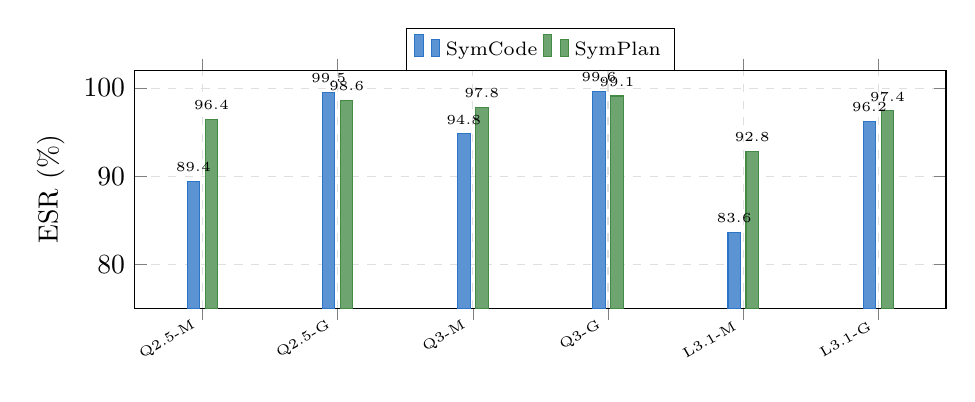
\begin{tikzpicture}
\begin{axis}[
    ybar,
    bar width=4.5pt,
    width=0.98\columnwidth,
    height=4.6cm,
    ymin=75,
    ymax=102,
    ylabel={ESR (\%)},
    symbolic x coords={Q2.5-M,Q2.5-G,Q3-M,Q3-G,L3.1-M,L3.1-G},
    xtick=data,
    nodes near coords,
    nodes near coords style={font=\tiny},
    legend style={at={(0.5,1.18)}, anchor=north, legend columns=-1, font=\scriptsize},
    grid=major,
    grid style={dashed, gray!25},
    x tick label style={font=\tiny, rotate=30, anchor=east}
]
\addplot[fill=accentblue!70, draw=accentblue!90] coordinates {(Q2.5-M,89.40) (Q2.5-G,99.50) (Q3-M,94.80) (Q3-G,99.60) (L3.1-M,83.60) (L3.1-G,96.20)};
\addplot[fill=checkgreen!70, draw=checkgreen!90] coordinates {(Q2.5-M,96.40) (Q2.5-G,98.60) (Q3-M,97.80) (Q3-G,99.10) (L3.1-M,92.80) (L3.1-G,97.40)};
\legend{SymCode, SymPlan}
\end{axis}
\end{tikzpicture}
\caption{Execution Success Rate (ESR) across models and benchmarks. M and G denote MATH-500 and GSM8K, respectively.}
\label{fig:chart}
\end{figure}

The cross-model results expose a consistent limitation of monolithic program generation in small models. CoT exceeds SymCode on both benchmarks for all three backbones. The gaps are 6.08 and 1.28 percentage points for Qwen2.5-Coder-7B, 3.60 and 0.70 points for Qwen3-8B, and 7.60 and 2.40 points for Llama-3.1-8B on MATH-500 and GSM8K, respectively. Nevertheless, SymCode frequently obtains ESR values above 90\%, demonstrating that a runnable program can still encode an incorrect equation, omit a condition, or return the wrong quantity. This observation is consistent with the SymCode study, which reports that its gains depend strongly on the coding proficiency of the base model and that less code-optimized models may underperform prose-based reasoning~\cite{nezhad2025symcode}.

SymPlan achieves the highest accuracy for every evaluated backbone. Relative to CoT, its gains are 8.40 and 5.29 points for Qwen2.5-Coder-7B, 7.80 and 4.20 points for Qwen3-8B, and 8.50 and 6.40 points for Llama-3.1-8B. Qwen3-8B provides the strongest absolute results, reaching 79.60\% on MATH-500 and 94.80\% on GSM8K, while Llama-3.1-8B produces the lowest scores across methods. Importantly, the SymPlan improvement persists across all three models, suggesting that representation and planning reduce the formulation burden before code synthesis rather than merely exploiting the coding strength of one backbone.

Table~\ref{tab:levels} shows that SymPlan remains strongest across the reported difficulty levels. Among the baselines, however, the relative ordering is not uniform: SymCode leads CoT on MATH Level 1 and GSM8K Level 3, whereas CoT is stronger on the remaining levels. Thus, symbolic code is beneficial when the model forms the correct program, while free-form CoT can be more robust when code synthesis introduces additional failure opportunities. SymPlan reduces this sensitivity by fixing the representation and solution plan before code generation.

The subject-wise results in Table~\ref{tab:subjects} show that the improvements extend beyond the aggregate scores. On MATH-500, the largest gains over CoT occur in Intermediate Algebra and Geometry, where explicit equations and domain conditions are especially important. On GSM8K, the clearest improvements appear in Percentages \& Finance and Arithmetic. Geometry reaches the same ceiling as CoT, while SymPlan remains strongest or tied across all reported subjects.

\subsection{Ablation Study}

We ablate structured representation and algorithmic planning independently on both benchmarks and all three backbones to measure their individual and combined effects.

\begin{figure}[t]
\centering
% Provisional ablation values; replace with measured results.
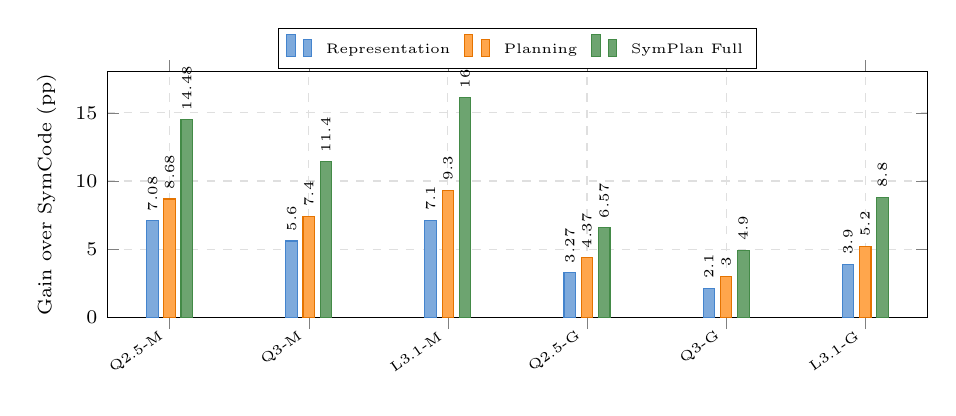
\begin{tikzpicture}
\begin{axis}[
    ybar,
    bar width=4.2pt,
    width=0.99\columnwidth,
    height=4.7cm,
    ymin=0,
    ymax=18,
    ylabel={Gain over SymCode (pp)},
    symbolic x coords={Q2.5-M,Q3-M,L3.1-M,Q2.5-G,Q3-G,L3.1-G},
    xtick=data,
    enlarge x limits=0.09,
    grid=major,
    grid style={dashed, gray!25},
    x tick label style={font=\tiny, rotate=35, anchor=east},
    y tick label style={font=\scriptsize},
    label style={font=\scriptsize},
    nodes near coords,
    nodes near coords style={font=\tiny, rotate=90, anchor=west},
    legend style={
        at={(0.5,1.18)},
        anchor=north,
        legend columns=3,
        font=\tiny,
        column sep=3pt
    }
]
\addplot[fill=accentblue!55, draw=accentblue!80] coordinates {
    (Q2.5-M,7.08) (Q3-M,5.60) (L3.1-M,7.10)
    (Q2.5-G,3.27) (Q3-G,2.10) (L3.1-G,3.90)
};
\addplot[fill=orange!70, draw=orange!90!black] coordinates {
    (Q2.5-M,8.68) (Q3-M,7.40) (L3.1-M,9.30)
    (Q2.5-G,4.37) (Q3-G,3.00) (L3.1-G,5.20)
};
\addplot[fill=checkgreen!70, draw=checkgreen!90] coordinates {
    (Q2.5-M,14.48) (Q3-M,11.40) (L3.1-M,16.10)
    (Q2.5-G,6.57) (Q3-G,4.90) (L3.1-G,8.80)
};
\legend{Representation,Planning,SymPlan Full}
\end{axis}
\end{tikzpicture}
\caption{Accuracy gains over SymCode~\cite{nezhad2025symcode} in the component ablation. M and G denote MATH-500 and GSM8K, respectively; single-component variants retain only representation or planning.}
\label{fig:ablation}
\end{figure}

Fig.~\ref{fig:ablation} shows that both components improve over SymCode~\cite{nezhad2025symcode} for every model--dataset pair, with planning providing the stronger individual variant in all six settings. The full pipeline achieves the highest accuracy throughout. Relative to SymCode, its gains are 14.48 and 6.57 points for Qwen2.5-7B, 11.40 and 4.90 points for Qwen3-8B, and 16.10 and 8.80 points for Llama3.1-8B on MATH-500 and GSM8K, respectively. The larger improvements on MATH-500 suggest that explicit representation and planning are especially useful when problems require longer symbolic transformations and stricter constraint handling. Their consistent combination gains indicate complementary roles: representation stabilizes the mathematical state, whereas planning organizes that state into an executable solution strategy.

\subsection{Error Analysis and Qualitative Examples}

The paired Level-5 logs provide direct evidence for the central hypothesis of this work. On the same 134 MATH-500 problems, CoT answers 56 correctly (41.79\%), whereas SymCode answers 48 correctly (35.82\%). SymCode nevertheless executes successfully on 110 problems, corresponding to an ESR of 82.09\%. Among these successful executions, 62 (56.36\%) still produce an incorrect answer, and 21 incorrect outputs are even accepted by the lightweight verifier. Thus, execution success primarily measures program validity, not whether the generated program represents the intended mathematics.

\begin{figure}[t]
\centering
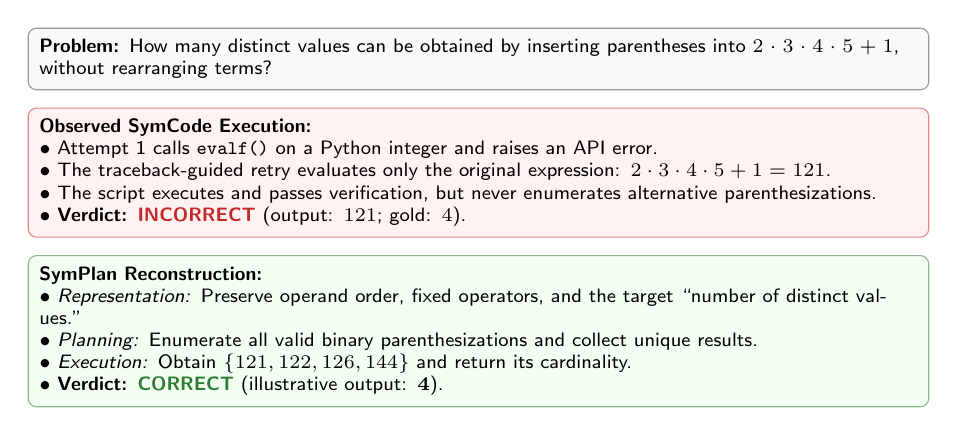
\begin{tikzpicture}[
    node distance=0.22cm,
    font=\sffamily\scriptsize,
    casebox/.style={draw=black!40, fill=boxgray, rounded corners=3pt,
                    text width=0.92\columnwidth, inner sep=4pt}
]

\node[casebox] (prob) {
    \textbf{Problem:} How many distinct values can be obtained by inserting parentheses into $2\cdot3\cdot4\cdot5+1$, without rearranging terms?
};

\node[casebox, below=of prob, draw=crossred!55, fill=red!5] (symcode) {
    \textbf{Observed SymCode Execution:}\\
    $\bullet$ Attempt 1 calls \texttt{evalf()} on a Python integer and raises an API error.\\
    $\bullet$ The traceback-guided retry evaluates only the original expression: $2\cdot3\cdot4\cdot5+1=121$.\\
    $\bullet$ The script executes and passes verification, but never enumerates alternative parenthesizations.\\
    $\bullet$ \textbf{Verdict:} \textcolor{crossred}{\textbf{INCORRECT}} (output: $121$; gold: $4$).
};

\node[casebox, below=of symcode, draw=checkgreen!55, fill=green!5] (symplan) {
    \textbf{SymPlan Reconstruction:}\\
    $\bullet$ \textit{Representation:} Preserve operand order, fixed operators, and the target ``number of distinct values.''\\
    $\bullet$ \textit{Planning:} Enumerate all valid binary parenthesizations and collect unique results.\\
    $\bullet$ \textit{Execution:} Obtain $\{121,122,126,144\}$ and return its cardinality.\\
    $\bullet$ \textbf{Verdict:} \textcolor{checkgreen}{\textbf{CORRECT}} (illustrative output: $\mathbf{4}$).
};

\end{tikzpicture}
\caption{A successful execution does not imply a correct mathematical formulation. The SymCode behavior is taken from the Level-5 log; the SymPlan path is a qualitative reconstruction.}
\label{fig:parenthesization_case}
\end{figure}

\textbf{Repairing execution without repairing meaning.} Fig.~\ref{fig:parenthesization_case} shows that traceback feedback repairs the API failure but leaves the semantic error untouched. The retry produces executable code by simplifying the task into direct evaluation, whereas representation and planning preserve the combinatorial target before code synthesis.

\textbf{Preserving structural conditions.} For the degree-5 interpolation problem with $p(n)=n/(n^2-1)$ for $n=2,\ldots,7$, SymCode produces an executable but unrelated polynomial construction and returns 39690 instead of $3/56$. The error is not numerical; the code fails to preserve the six interpolation constraints and the degree condition. A structured representation exposes these six exact point constraints, after which the plan can apply Lagrange interpolation or symbolic interpolation with rational arithmetic before evaluating $p(8)$.

\textbf{Maintaining variable semantics and domains.} For the number of real $x$ such that $\sqrt{120-\sqrt{x}}$ is an integer, SymCode runs successfully, returns 0, and passes verification because the verifier only checks that the output is a nonnegative integer. SymPlan instead introduces $n=\sqrt{120-\sqrt{x}}\in\mathbb{Z}_{\ge0}$, derives $\sqrt{x}=120-n^2\ge0$, and obtains $n\in\{0,\ldots,10\}$. This yields 11 valid values of $x$, while making the domain conditions explicit before code generation.

These cases explain why CoT can outperform monolithic SymCode on compact models despite SymCode's high ESR. Traceback-guided repair is effective for syntax, API, and type failures, but it cannot reliably detect a runnable program that encodes the wrong target, transformation, or constraint. The reconstructed SymPlan examples illustrate the intended mechanism: representation stabilizes the mathematical state, planning selects a valid transformation sequence, and symbolic execution is used only after these decisions have been made. These illustrative SymPlan outputs should be replaced or confirmed when the corresponding runs finish.

\FloatBarrier

\section{Conclusion}

In this paper, we presented SymPlan, a structured neurosymbolic framework for mathematical reasoning in compact open-weight language models. By separating formal problem representation from algorithmic planning before plan-guided SymPy generation, SymPlan addresses semantic misformulation and constraint omission through an explicit reasoning pipeline. The generated program carries the extracted constraints into Python execution, with interpreter tracebacks supporting correction when execution fails. Evaluations on MATH-500 and GSM8K demonstrate higher mathematical accuracy while maintaining high execution reliability, without parameter fine-tuning.

In future work, we plan to extend SymPlan to multimodal mathematical reasoning involving geometric diagrams, as well as investigate the integration of interactive formal theorem provers (such as Lean) to verify open-ended deductive proofs on edge devices.

\balance
\bibliographystyle{IEEEtran}
\bibliography{cite}

\end{document}
